\documentclass[12pt,a4paper]{article}
\usepackage[margin=2cm]{geometry}
\usepackage{graphicx} % Required for including pictures
\usepackage{float} % Allows putting an [H] in \begin{figure} to specify the exact location of the figure
\usepackage{wrapfig} % Allows in-line images such as the example fish picture
\usepackage{color}
\usepackage{mathtools}
\usepackage{graphicx}
\usepackage{hyperref}
\usepackage{titling}
\usepackage{braket}
\usepackage{cancel}
\usepackage{acronym}
\usepackage{subcaption}
\usepackage{caption}
\usepackage[space]{grffile} % allows file names with spaces
\usepackage{lipsum}

\hypersetup{
colorlinks=true,
linkcolor=blue,
urlcolor=blue
}

\acrodef{stem}[STEM]{Scanning Transmission Electron Microscopy}
\acrodef{tem}[TEM]{Transmission Electron Microscope}
\acrodef{cemn}[CEMN]{Center for Electron Microscopy and Nanofabrication}
\acrodef{edx}[EDX]{Energy-dispersive X-ray spectroscopy}
\acrodef{sem}[SEM]{Scanning Electron Microscope}
% http://staff.science.uva.nl/~polko/HOWTO/LATEX/acronym.html 

%\setlength\parindent{0pt} % Uncomment to remove all indentation from paragraphs

\graphicspath{{Data/}} % Specifies the directory where pictures are stored

\title{TEM Report 2}
\author{Bret Comnes}
\date{\today}
\posttitle{\par\end{center}}
\setlength{\droptitle}{-10pt}


\begin{document}

\maketitle

\section{Introduction} % Major section

This report will cover some basics concepts relating to \ac{stem} and \ac{edx}, as well as some simple analysis of data taken a student lab session at the \ac{cemn} at Portland State University on May 16, 2014.  Bright field \ac{stem} images, \ac{edx} data and point spectrum of the inspected sample are included.  The data was collected using a FEI Technai \ac{tem} and the accompanying AZtec EDS acquisition and analysis tool.

Spectrum analysis is performed using latest version of Fityk\cite{ft}: v.1.2.9.  Additional work was performed to build newer versions of Fityk from source and add it to the Homebrew\cite{home} package manager for future convenience of other students and researches.


\section{\ac{stem} Fundamentals} % (fold)
\label{sec:stem}

\ac{stem} uses the formation of a fine point of electrons rastering across the sample to provide information about specific points of the specimen.  This allows for mapping of \ac{edx} to specific points of the sample as well as limiting radiation exposure to smaller well defined sections of the sample.  Scanning coils are used to horizontally scan the beam across the surface as apposed to pivoting around a point like you would find in an \ac{sem}.

Because \ac{stem} images are formed by a raster scan, instead of using lenses to form an image, we no longer have to worry about defects in our lenses which can cause issues like chromatic aberration in thick samples.  Magnification of \ac{stem} images are determined by scan geometry.  While \ac{stem} can provide better contrast, images tend to be noisier than \ac{tem} mode images.  \cite{tem}  

\ac{stem} can generate both bright field and dark field images.  \ac{stem} actually provides images with less noise and better contrast than \ac{tem} but at the cost of lower resolution.  This can be useful for thick or unstained samples which provide very little image details and require the higher contrast \ac{stem} provides.  \ac{stem} gives more flexibility over the contrast of images because it allows control over things like detector gain and contrast/brightness settings that are not available on the analog \ac{tem} screen  (however you can always digitalis images from the normal \ac{tem} mode and apply post processing to your images to enhance contrast).  

\section{\ac{edx} fundamentals} % (fold)
\label{sec:edx}

\ac{edx} allows for detection of the chemical composition of samples.  It can be used with \ac{stem} to map chemical composition to specific locations on the sample.  Electrons are a type of ionizing radiation, meaning, that it can cause inner shell electrons in the sample to be ejected, resulting in secondary signals that contain useful information.  \ac{edx} uses the secondary X-rays ejected due to \ac{tem} radiation to plot the characteristic peaks of the elements contained within a sample.   

\ac{edx} is a form of spectroscopy, so detects and distinguishes x-rays by their energy level.  This is critical for the function of \ac{edx} as the whole point is to determine chemical composition.  Typical detectors are made out of $Si(Li)$.

Spectra can be acquired in a few common ways.  Spot mode uses the \ac{tem} to collect spectra from one particular point or feature.  This method is basic and can be time consuming if you have to gather spectra from a wide area or set of features.  It is also subject to operator bias as you may fail to check certain sections of the sample that don't look interesting.   A variation of this method can be done as a line profile.  Dot mapping scans the sample and maps detections to the sample image for a given wavelength.  This method can be augmented with post processing to provide false coloring to the image.  Finally there is spectrum imaging that allows us to collect a full spectrum of x-rays at every pixel.  This, unsurprisingly, uses \ac{stem} mode.

It isn't a matter of simple detecting x-rays as there are all sorts of sources of background noise and other peaks that exist due to other phenomena.  Issues arise due to high voltage electrons in the illumination system that generate large does of undesired x-rays as well as to scattering off very thin samples.  One can also have issues with spurious x-rays, which are generated by the sample, but not from the desired region, showing up in the spectra.
% section acedx_fundamentals (end)

\section{Data Analysis} % (fold)
\label{sec:data_analysis}

We collected bright field TEM images of a Iron Oxide ($Fe_3O_4$) particles coated with Silicon dioxide ($SiO_2$).  Additionally, we collected \ac{edx} spectrum information and mapped the location of these different elements using the AZtec software.  The data was explored in a limited manner use the Fityk software.  Unfortunately the \ac{stem} images were lost in the process of exporting data and cannot be included.

\subsection{TEM imaging} % (fold)
\label{sub:tem_imaging}

Bright field images of Iron Oxide particles coated with Silicon dioxide were taken.  \ac{tem} imaging consists of illuminating thin samples that are semi electron transparent with a focused electron beam to project an image of the sample onto a viewing screen or camera.

\begin{figure}[htbp]
  \centering
  
  \begin{subfigure}[b]{0.45\textwidth}
    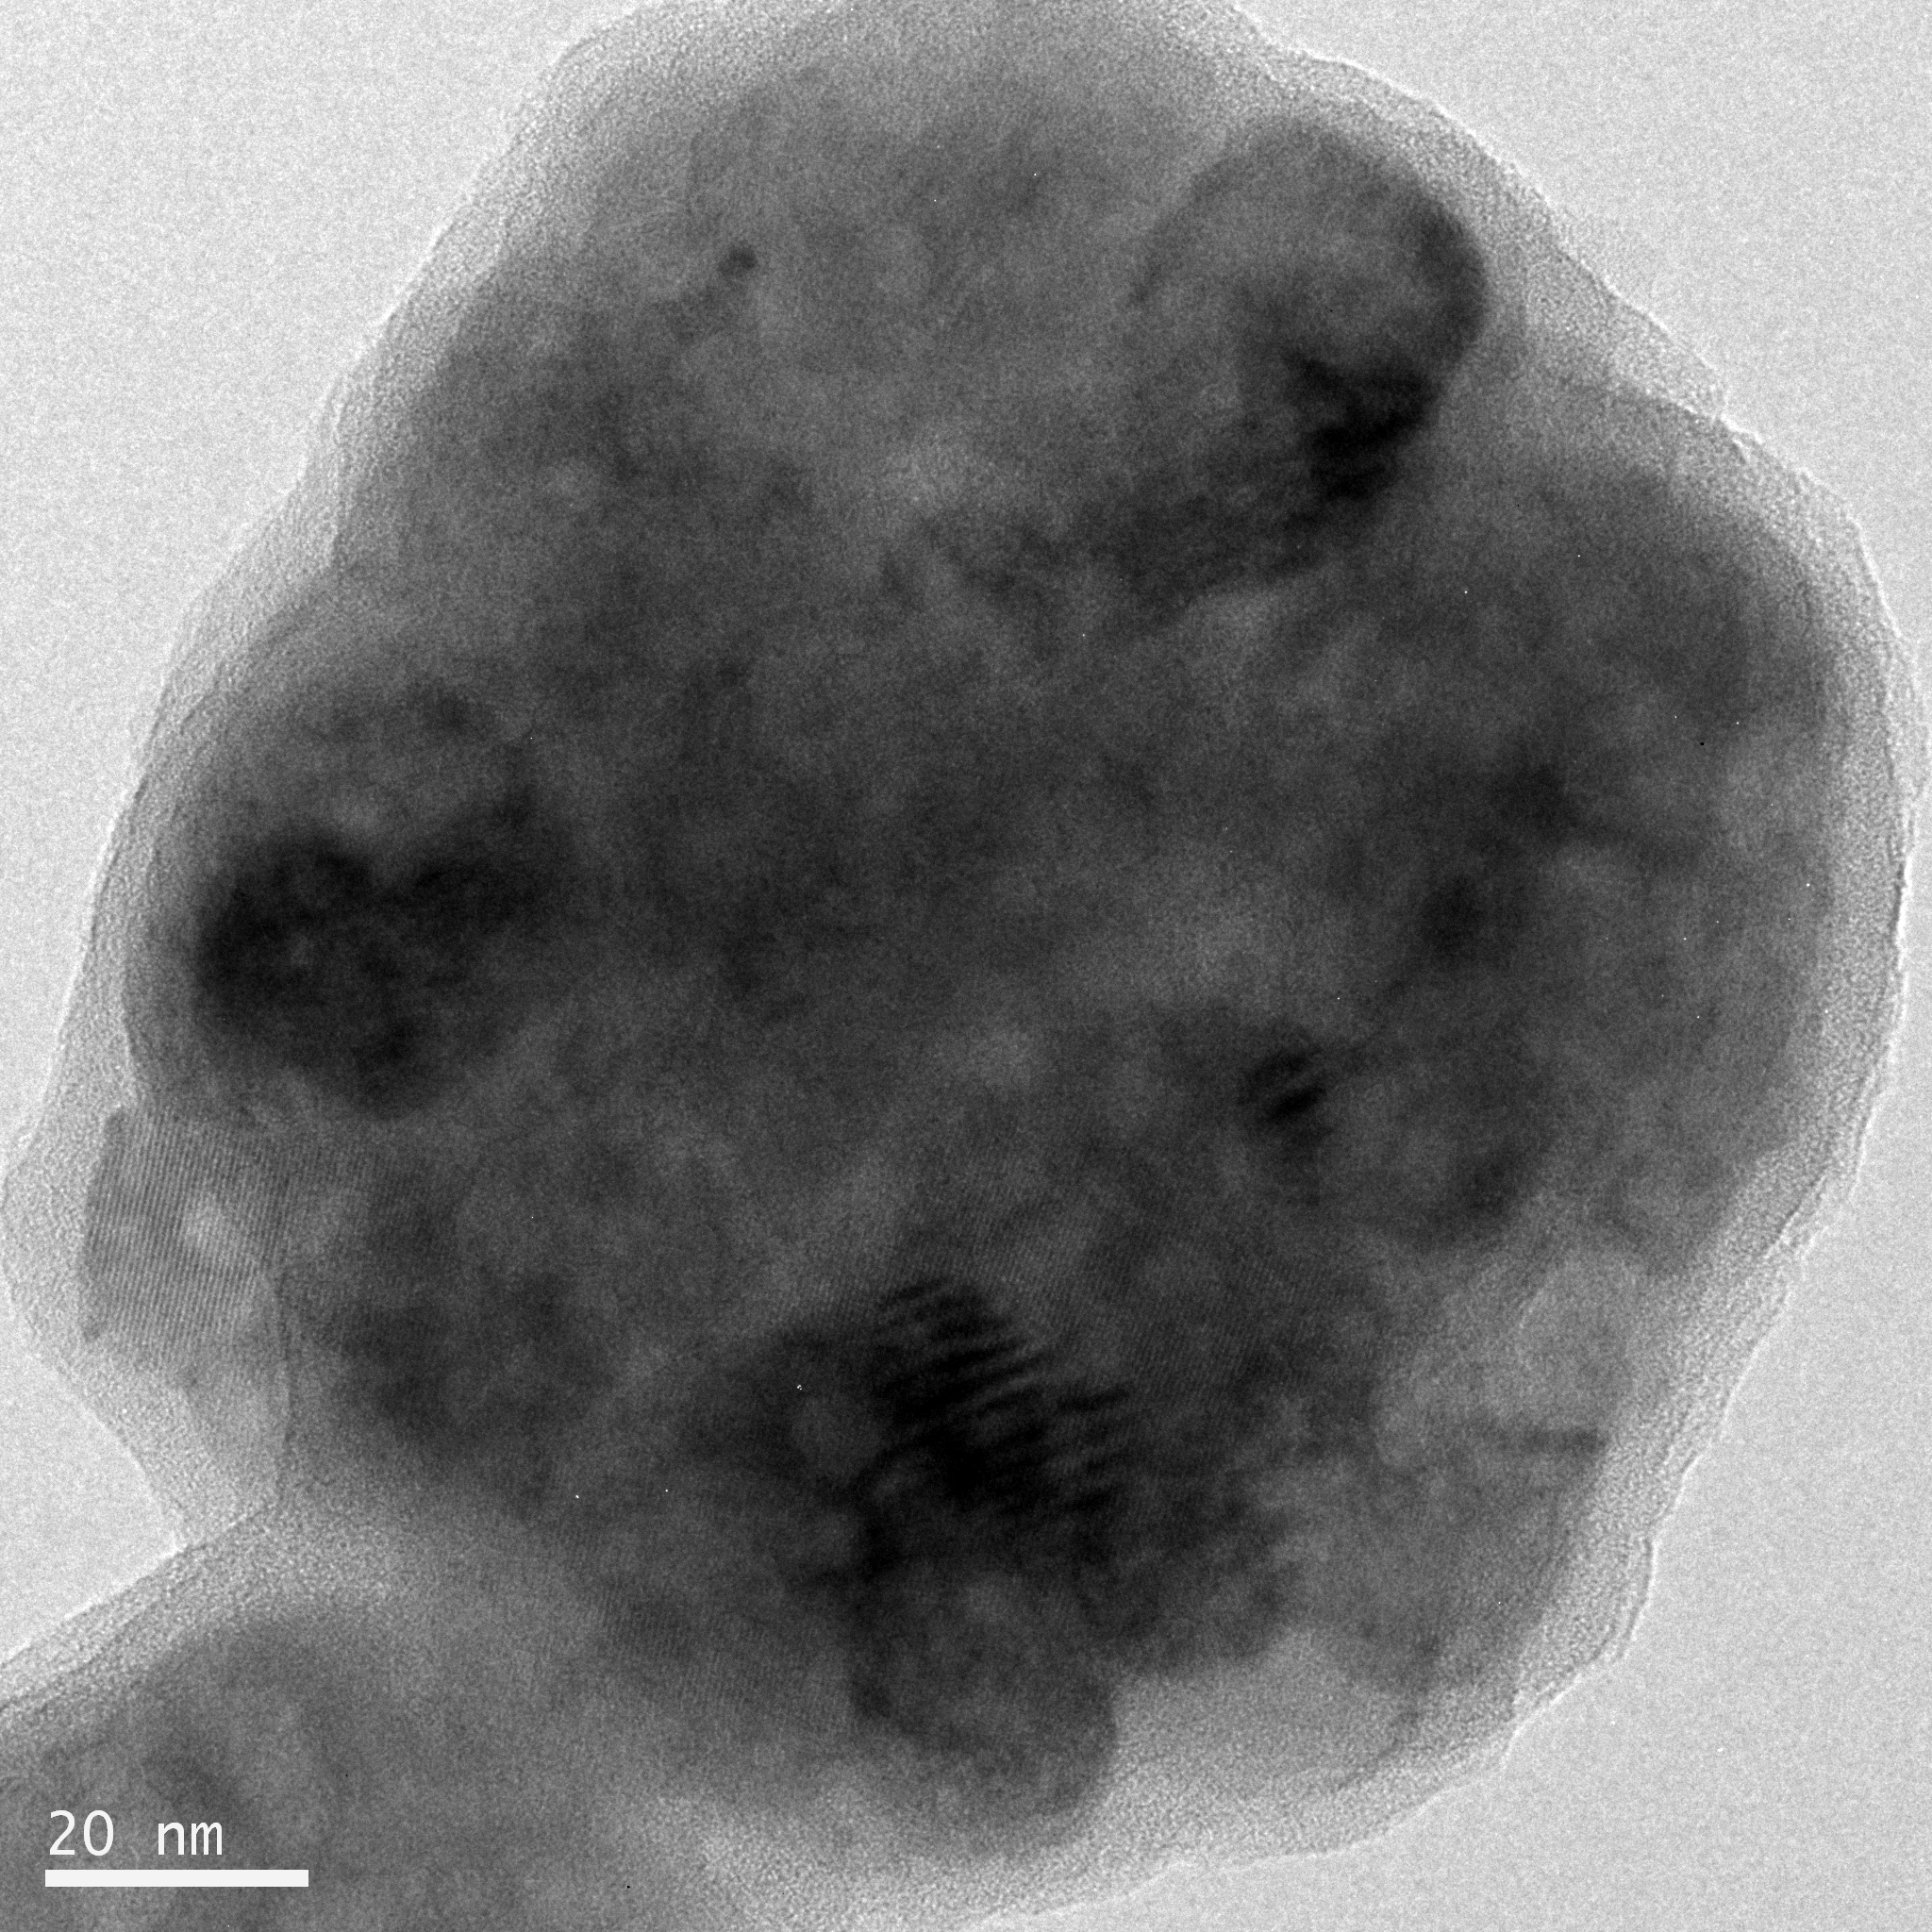
\includegraphics[width=\textwidth]{Data/Fe3O4-SiO2-0001.png}
  \end{subfigure}%
  \begin{subfigure}[b]{0.45\textwidth}
    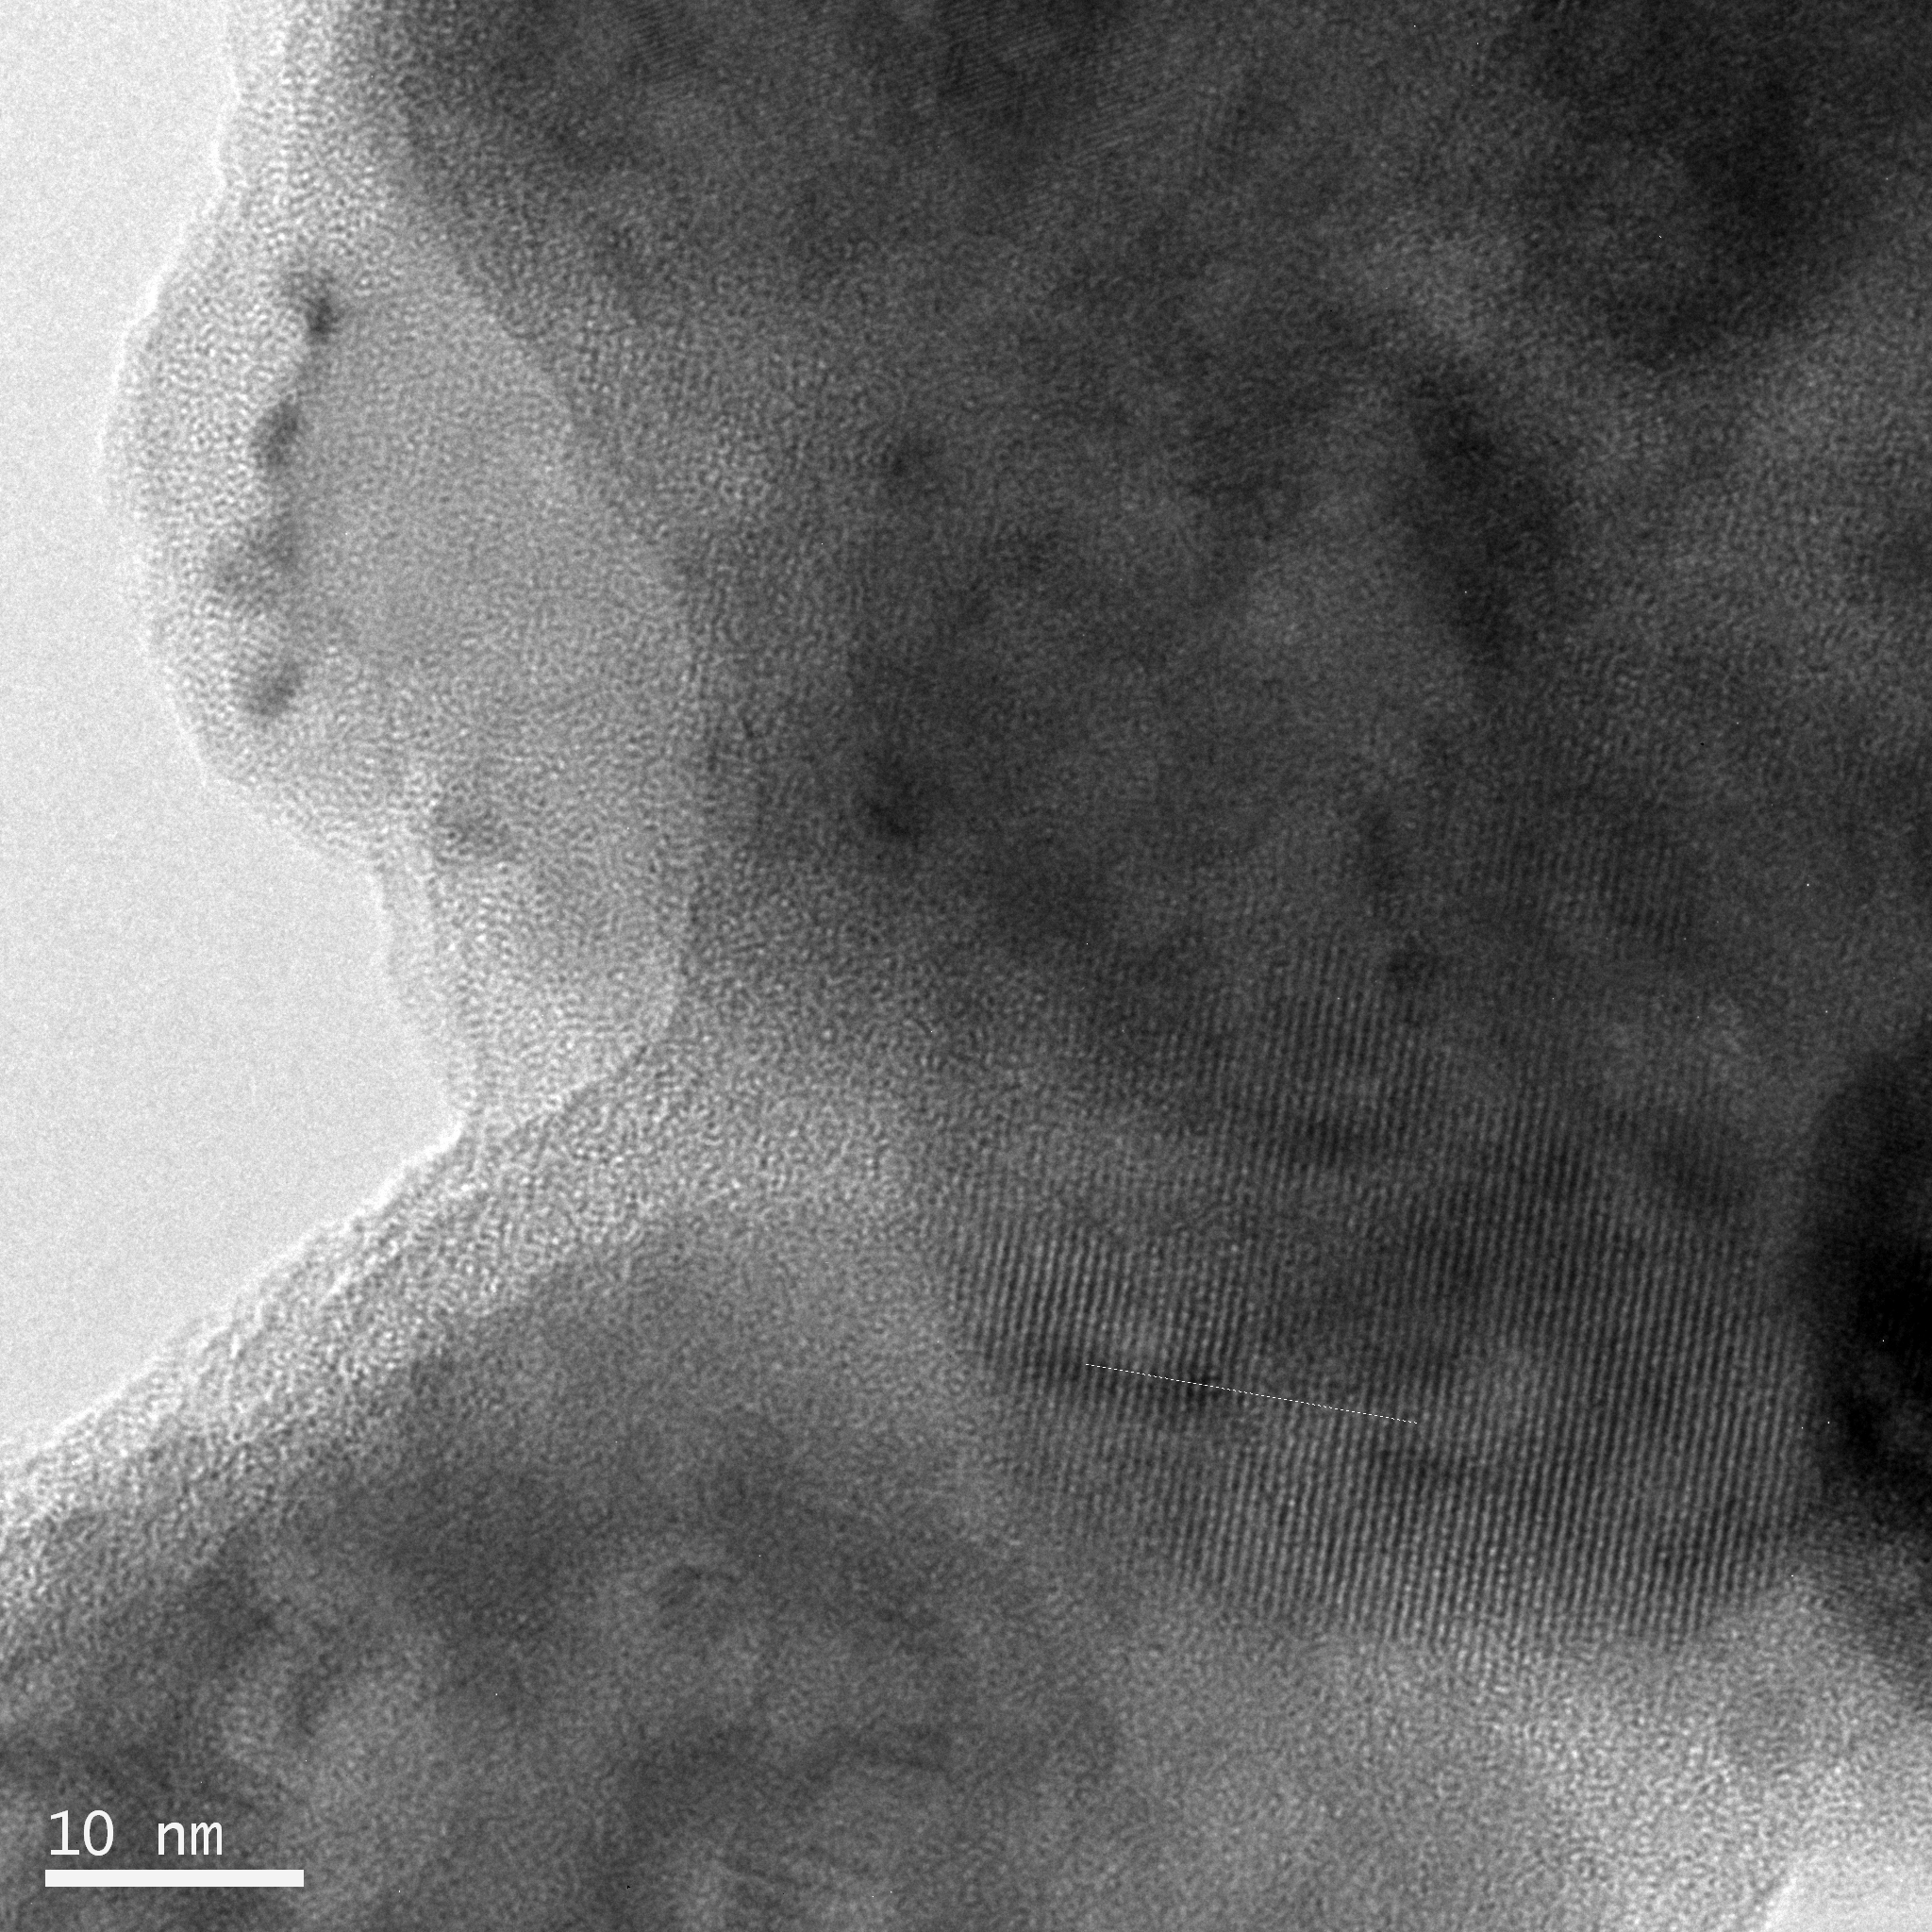
\includegraphics[width=\textwidth]{Data/Fe3O4-SiO2-0002.png}
  \end{subfigure}
  
  \begin{subfigure}[b]{0.45\textwidth}
    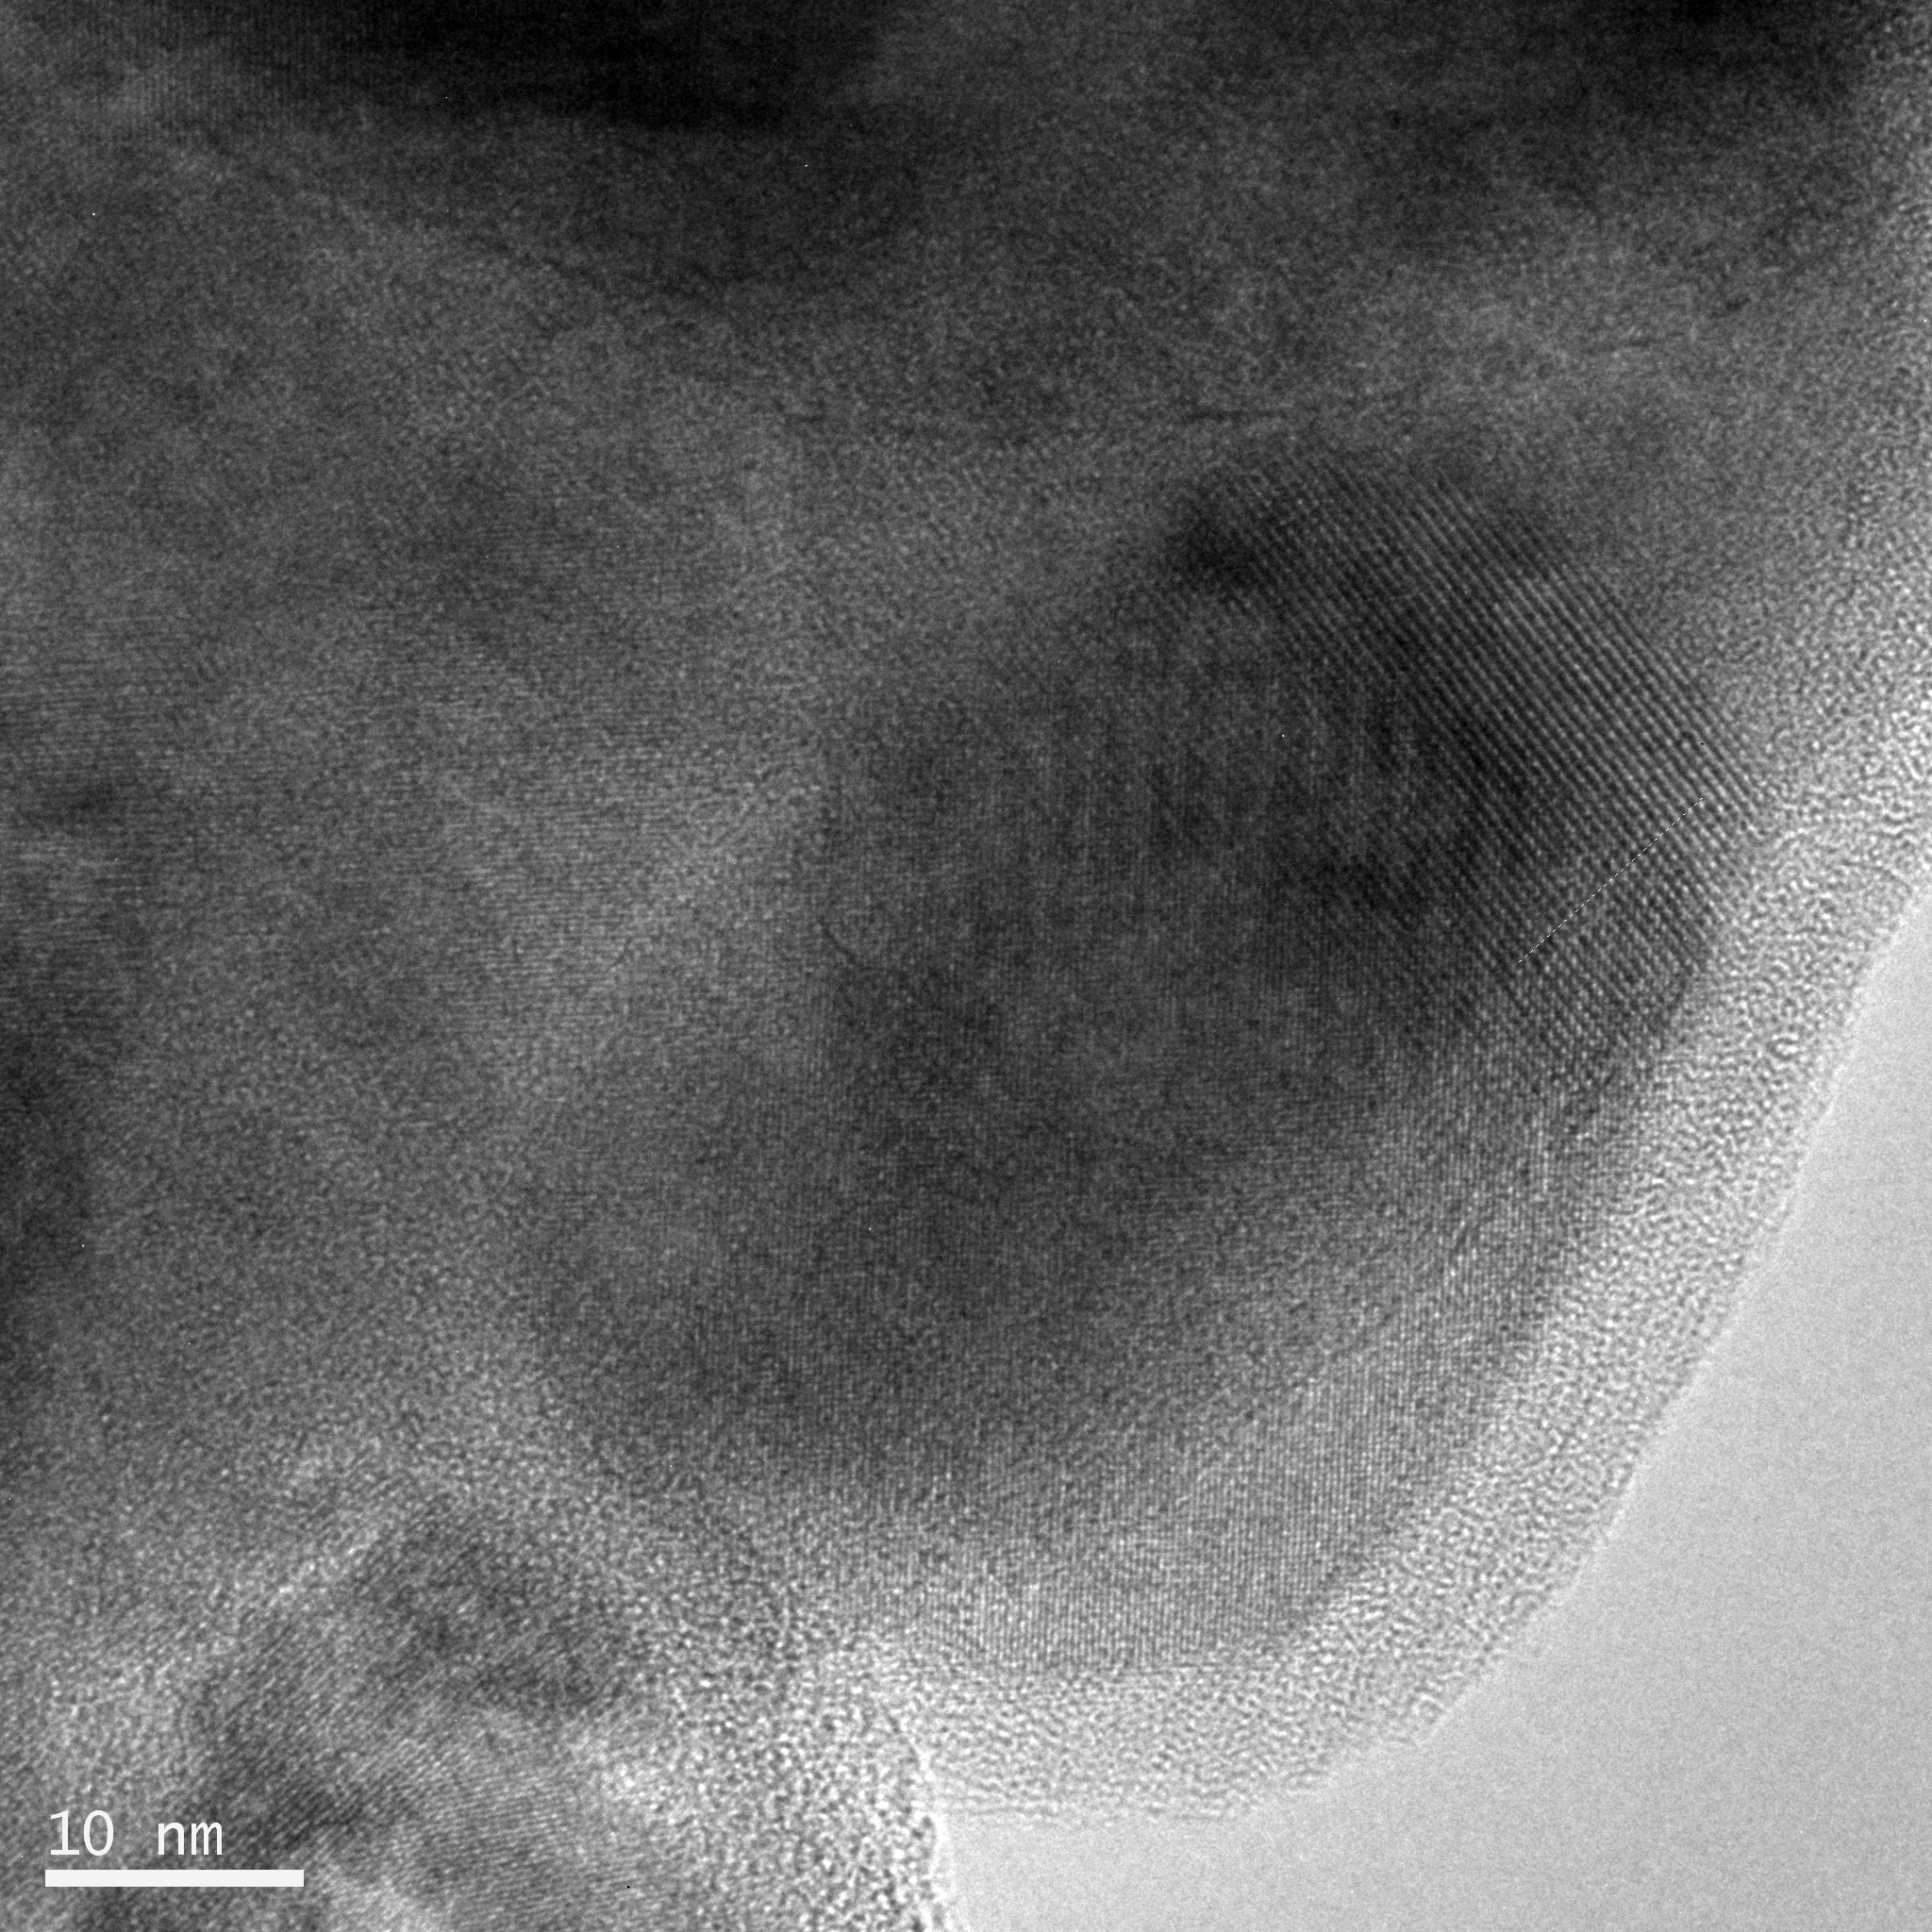
\includegraphics[width=\textwidth]{Data/Fe3O4-SiO2-0003.png}
    \caption{Visible lattice pattern}
    \label{fig:viewc}
  \end{subfigure}
  \begin{subfigure}[b]{0.45\textwidth}
    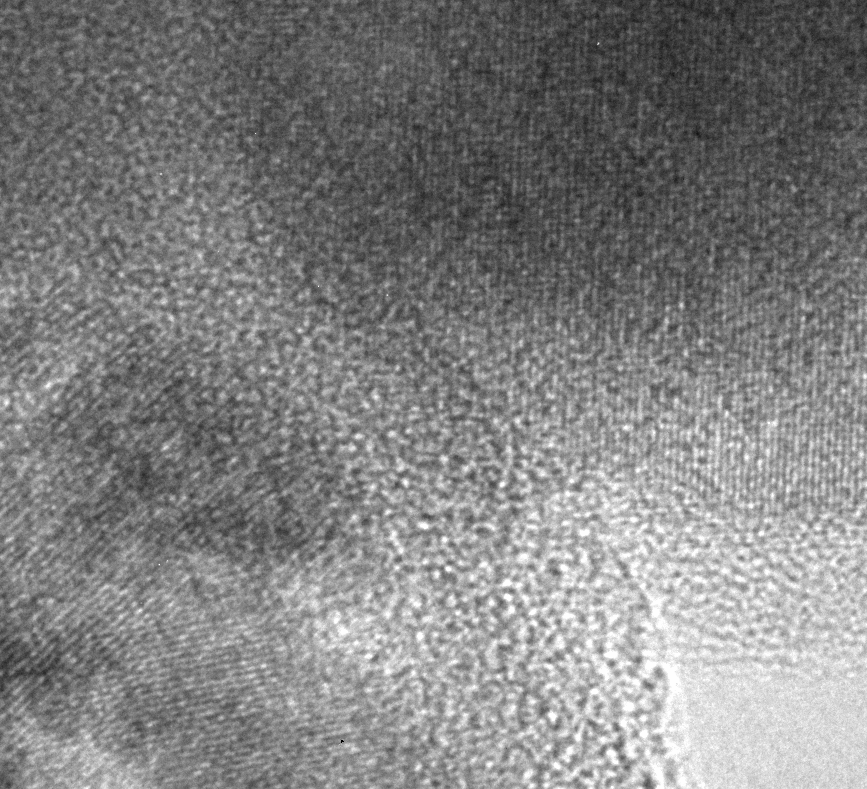
\includegraphics[width=\textwidth]{Data/Fe3O4-SiO2-0003-zoom.png}
    \caption{Magnified view of \ref{fig:viewc}.  }
    \label{fig:zoom}
  \end{subfigure}
  
  \caption{Various views of Bright field Images of $SiO_2$ coated $Fe_3O_4$ particles}\label{fig:brightfield}
\end{figure}

The images in Figure~\ref{fig:brightfield} show an incredible level of detail and magnification.  It is important to understand what you are looking at in order to properly interpret an image.  We are typically used seeing images of 3D objects reflecting light back into a detector (a camera or our eyes).  This is typical of a \ac{sem} image.  Remember that \ac{tem} images are 2D images of 3D objects generated by transmitting light through the sample (rather than off of it).  Take this into account when observing these details.

Some interesting features that are visible are the crystal lattice lines of the particle.  They are particular apparent in Figure~\ref{fig:zoom}.  Bringing the image into focus and then slightly out of focus provides the clearest image and level of contras needed to 

% subsection tem_imaging (end)

\subsection{EDX Spectroscopy} % (fold)
\label{sub:edx_spectroscopy}

The \ac{edx} spectrum was collected of our sample using the AZtec software.  An image of this can be seen in Figure~\ref{fig:aztec}.  This data was replotted and fitted in Fityk and is shown in in Figure~\ref{fig:fitk}.  

The two spectrum plots look very similar.  It seems like AZtec is doing some kind of post processing to the data.  The curve fit is generated automatically and the identification labels are conveniently applied for us.  The main difference between the two representations of the data is the peak missing around 0 in the AZtec plot, that is present in the Fityk plot.  I'm fairly sure this is a background signal that AZtec is suppressing.  We see a tall peak for $O$ next to a peak for $Fe$.  A close up of these peaks can be seen in Figure~\ref{fig:cross} where fitting the data in Fityk shows a super position peak between these two main peaks.  Pretty great!  

There is a small peak identified by the AZtec software for $Cu$ next to these peaks, but this was barely   visible.  Further on we see our $Si$ peak loud and clear

Further out on the spectra (Figure~\ref{fig:outer}) we see a strong peak and weaker peak for $Fe$ as well as a peak for $Cu$.  There is one additional peak that appears in our Fityk plot that isn't seen in the AZtec view.  This is possibly due to a limited view on the AZtec software or the fact that this outer peak is so negligible that it isn't worth noting.  The $Cu$ peaks are expected as our sample holder is made out of copper so this accounts and confirms our preexisting understanding of the composition of our sample!

\begin{wrapfigure}{r}{0.5\textwidth}
  \begin{subfigure}[b]{0.5\textwidth}
    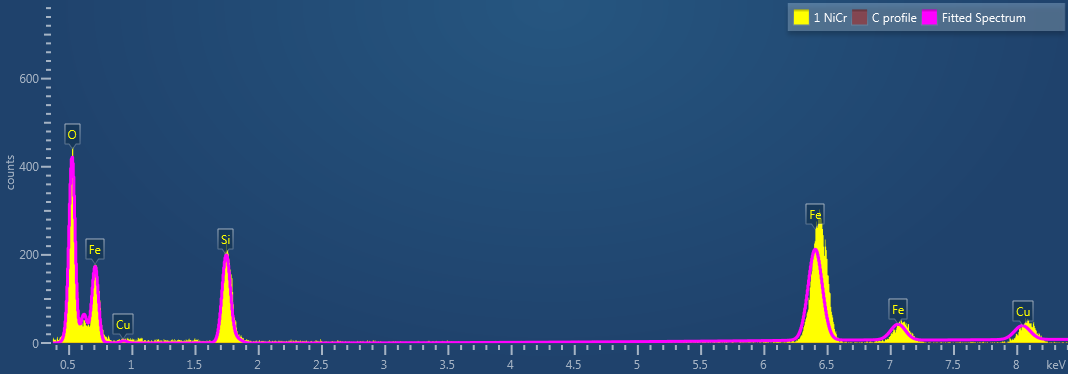
\includegraphics[width=\textwidth]{Data/EDS Spectrum.png}
    \caption{EDX Spectrum from AZtec}
    \label{fig:aztec}
  \end{subfigure}%

  \begin{subfigure}[b]{0.5\textwidth}
    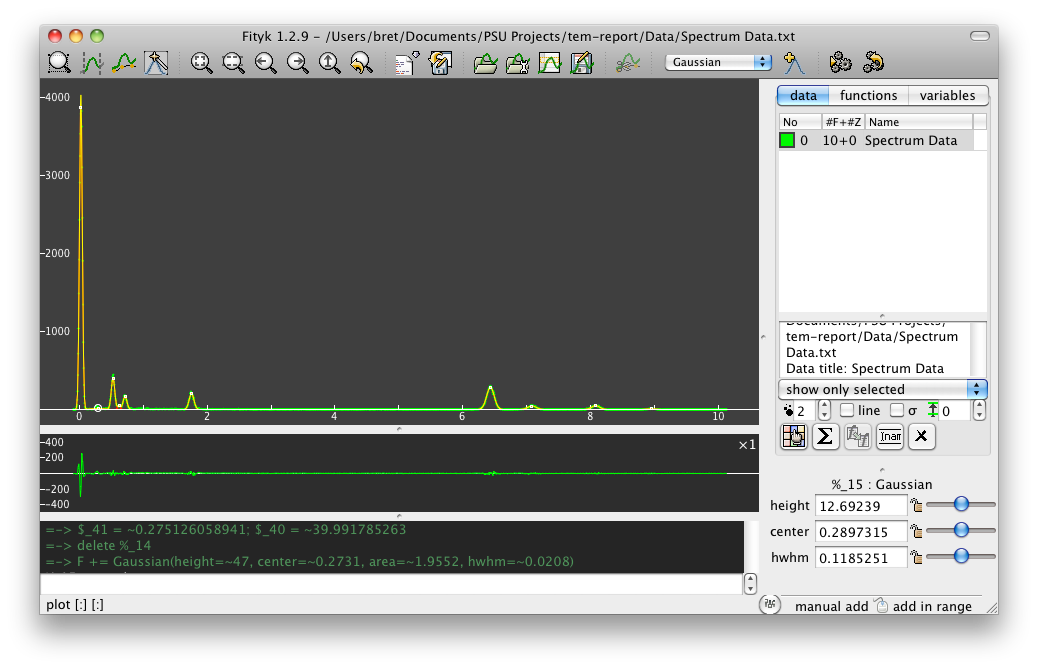
\includegraphics[width=\textwidth]{Data/full.png}
    \caption{Fitted EDX Spectrum from Fityk}
    \label{fig:fitk}
  \end{subfigure}%

  \caption{EDX Spectroscopy Data}
  \label{fig:edx}
\end{wrapfigure}

\begin{figure}[htbp]
  \centering
    \begin{subfigure}[b]{0.45\textwidth}
    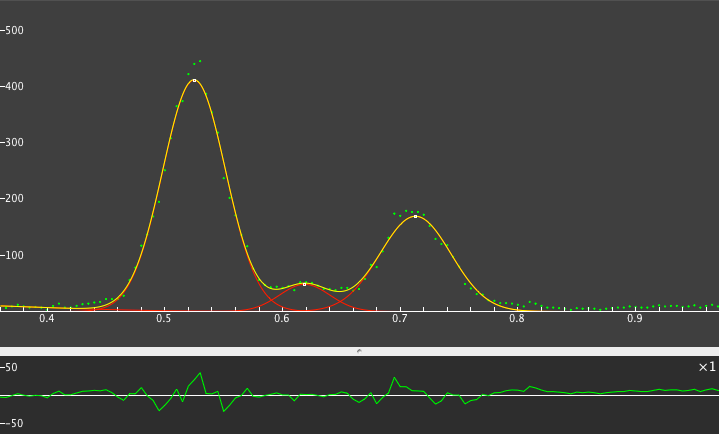
\includegraphics[width=\textwidth]{Data/crossover.png}
    \caption{False peak between $O$ and $Fe$ peaks.}
    \label{fig:cross}
  \end{subfigure}
  ~
  \begin{subfigure}[b]{0.45\textwidth}
    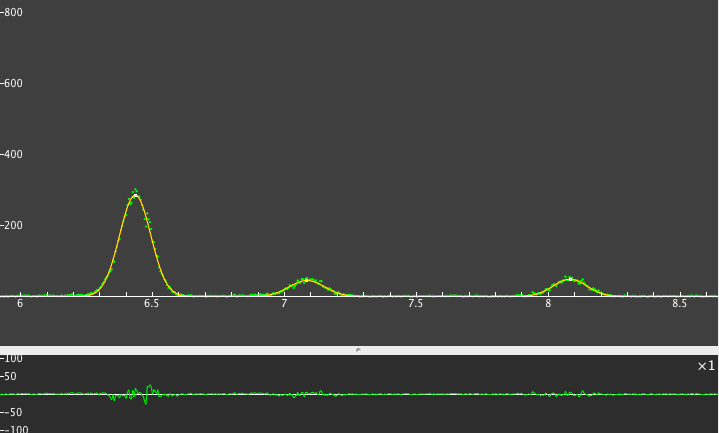
\includegraphics[width=\textwidth]{Data/outer_peak.png}
    \caption{Close up of outer $Fe$ and $Cu$ peaks.}
    \label{fig:outer}
  \end{subfigure}%
  \caption{Close up of fitted data in Fityk}
  \label{fig:fit}
\end{figure}

% subsection edx_spectroscopy (end)

\subsection{EDS Maps} % (fold)
\label{sub:eds_maps}

\begin{figure}[htbp]
  \centering
  \begin{subfigure}[b]{0.35\textwidth}
    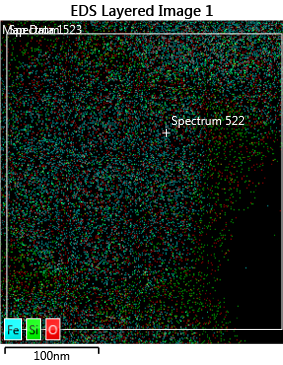
\includegraphics[width=\textwidth]{Data/Map.png}
    \caption{Composite Element Map}
    \label{fig:map}
  \end{subfigure}
  \begin{subfigure}[b]{0.35\textwidth}
    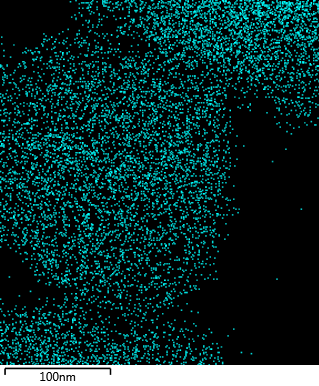
\includegraphics[width=\textwidth]{Data/Fe Map.png}
    \caption{Map of $Fe$}
    \label{fig:fe_map}
  \end{subfigure}
  
  \begin{subfigure}[b]{0.35\textwidth}
    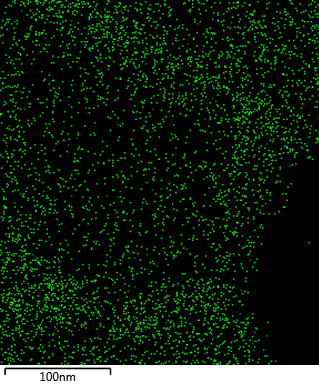
\includegraphics[width=\textwidth]{Data/Si Map.png}
    \caption{Map of $Si$}
    \label{fig:si_map}
  \end{subfigure}
  \begin{subfigure}[b]{0.35\textwidth}
    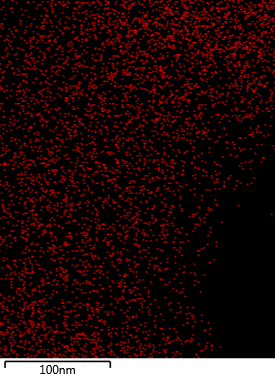
\includegraphics[width=\textwidth]{Data/O Map.png}
    \caption{Map of $O$}
    \label{fig:o_map}
  \end{subfigure}
  \caption{EDX Maps of Particle Sample}\label{fig:map_grid}
\end{figure}

The \ac{edx} maps are shown in Figure~\ref{fig:map_grid}.  Unfortunately the underlying \ac{stem} image that could be superimposed below these maps was not preserved during export.  It was, however, similar to images seen in Figure~\ref{fig:brightfield} which can give a feel for the overall structure of the particles.  From these bright field images, note the darker inner structure which appears surrounded by a more transparent outer layer.

These maps are generated using \ac{edx} readings for different wavelengths at different positions on our sample.  This is done by imaging in \ac{stem} mode and correlating the \ac{edx} reading to that particular pixel.

The composite map in Figure~\ref{fig:map} is a bit difficult to read but shows the mapping of all three elements: $Fe$, $Si$ and $O$ to the position on our sample.  It gives some idea of reading density, but it is still hard to see much underlying structure.

Figure~\ref{fig:fe_map} of the $Fe$ mapping gives the best picture of underlying structure although without the underlying \ac{stem} image it will require some imagination and comparison to Figure~\ref{fig:brightfield}.  The blue dots follow the shape of the darker inner structure of the particle, with a higher density of readings near the center indicating thickness of the particle near the center.  This daker core of the particle appears to be the $Fe$ and is consistent with our understanding of the sample wich is coated samples made up of $Fe$.

Looking that the map of $Si$ in Figure~\ref{fig:si_map}, we can see a larger outer structure which lines up with the more transparent coating around the darker inner core of the sample.  Its less dense around edges of the outer transparent section and less dense in the middle of the darker feature in the BF image.  It become most dense around the waist of the darker feature.  This seems to indicate that this might be a coating of some kind, with additional accumulation between the $Fe$ particles and not as tick at the cross section of the Iron particle.

Finally, the mapping of $O$ in Figure~\ref{fig:o_map} seems to be additive of both the $Fe$ detections and the $Si$ detections.  Its less dense around the edge of the outer surface ($Si$), becomes more dense when there is additional accumulation of $Si$ between the $Fe$ particles and the most dense around the $Fe$ particle covered in $Si$.  Perhaps this effect is purely additive due to the higher counts of both the $Fe_3O_4$ and $SiO_2$.
% subsection eds_maps (end)

% section data_analysis (end)

\section{Fityk Added to Homebrew} % (fold)
\label{sec:fityk_homebrew}

Upon discovering that newer Fityk versions were only offered as runnable binaries for paying subscriptions that required a hefty fee, a simple \texttt{ruby} formula was submitted as a pull request to the Homebrew Science repository\cite{hbs}.

\begin{wrapfigure}{r}{0.5\textwidth}
  \centering
  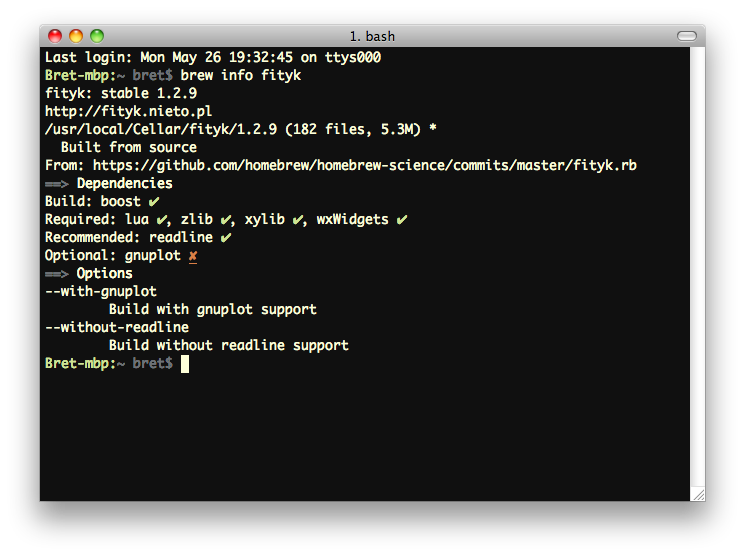
\includegraphics[width=0.5\textwidth]{Data/Screen shot 2014-05-26 at 7.33.21 PM.png}
  \caption{Homebrew Package Info on Fityk}
  \label{fig:homebrew}
\end{wrapfigure}

Homebrew\cite{home} is a popular 3rd party package manager for Mac OS X that manages the building and installation of open source software packages.  Upon the writing of this paper, the pull request was waiting for approval.  Discussions with maintainers about acceptance, however, sounded positive\cite{fpr}.  This will allow others to simply install the latest version of Fityk from the command line by running \texttt{\$ brew install fityk}.  A formula for the Fityk dependency, \texttt{xylib}, was also submitted to the \texttt{homebrew-science} repository\cite{xpr}. 

% section fityk_homebrew (end)

\section{Conclusion} % Major section

We successfully took bright field images of $SiO_2$ coated $Fe_3O_4$ particles featuring details of the crystal lattice structure, took \ac{edx} spectra confirming our understanding of the sample composition.  Finally we took a mapping of the sample composition using the \ac{tem} in \ac{stem} mode.  The data was explored somewhat additionally using the Fityk software and additional effort was exerted to increase accessibility to later versions of the Fityk software through the use of the Homebrew Package manager.

\bibliography{main} 
\bibliographystyle{plain} \nocite{*}

\end{document}